\section{System}



\subsection{Perturbation-Driven Exploration}
\label{sec:perturb}


\subsection{Attention Visualization}
As illustrated in Figure~\ref{fig:attention}(a)(b), the most widely adopted technique to bipartie graph

Attention matrix


\begin{figure*}[t]
\centering
\vspace{-2mm}
 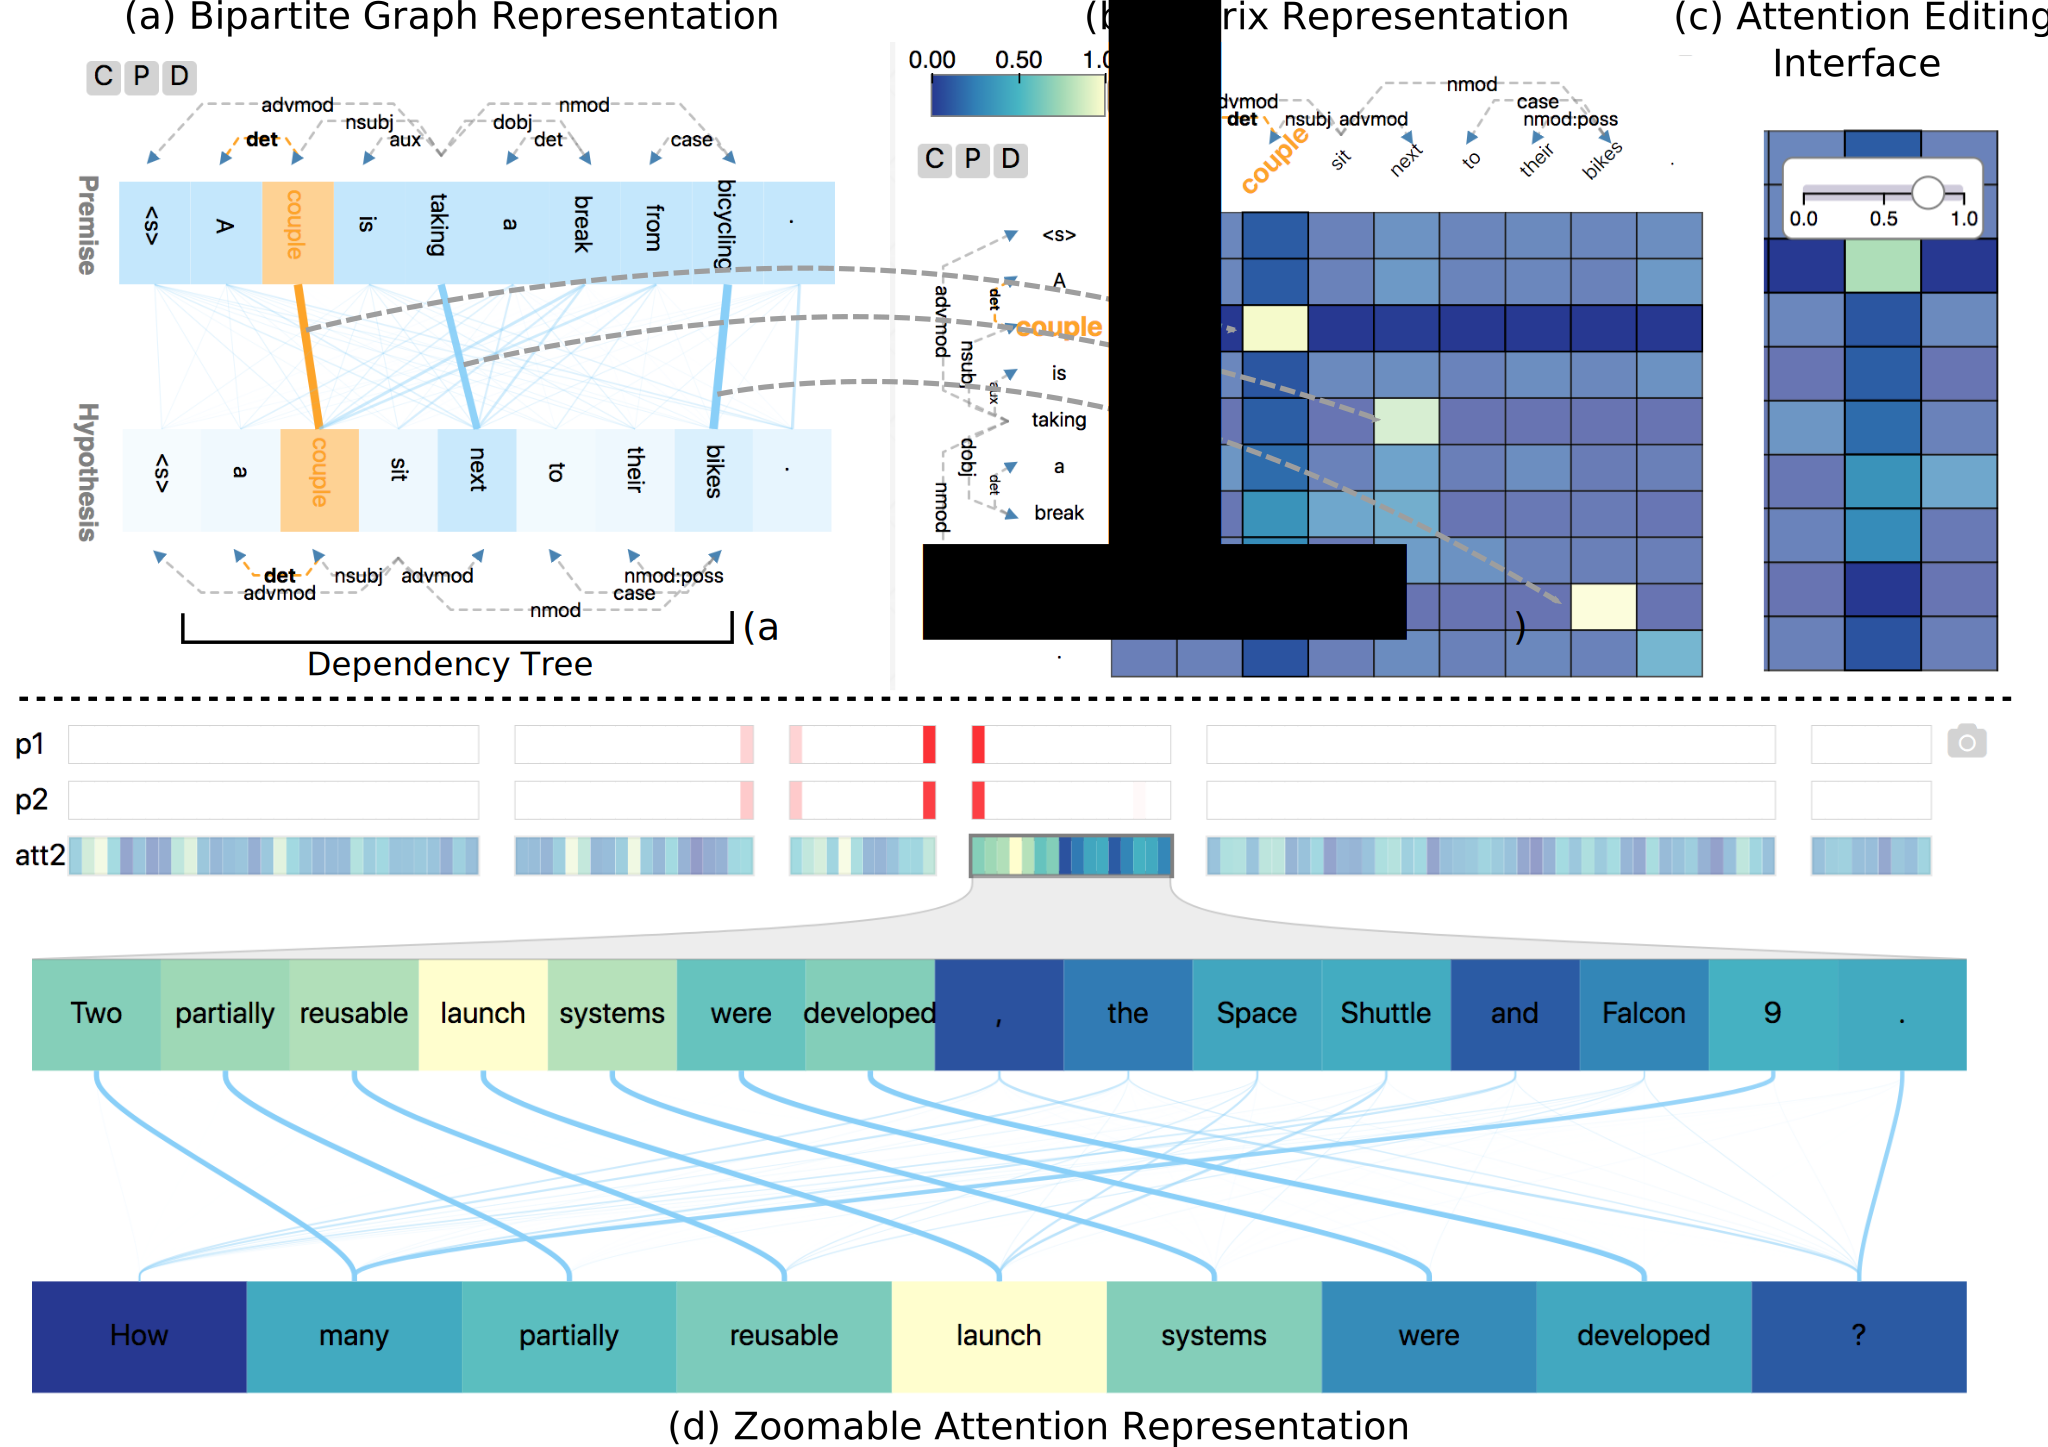
\includegraphics[width=1.0\linewidth]{attentionPanels}
  \vspace{-6mm}
 \caption{
Attention visualization. In the graph attention view (a), a bipartite graph encoding is adopted, in which the edge thickness corresponds to the attention value. In the matrix attention view (b), the entries of $i^{th}$ row represent the probabilities of words in hypotheses align to the $i^{th}$ word in the premise.
The user can alter the attention values via the pop-up interface illustrated in (c).
We overlay the dependency tree ($a_1$) grammar structure to highlight important words and allow simplification of complex sentence based on the dependency tree.
%
For highly asymmetric attention relationship, we utilized a zoomable hierarchical visual representation (d).
}
\label{fig:attention}
\end{figure*}


\subsection{Prediction Summarization}


\subsection{Implementation}
The initial setup cost and learning curve of the tool are often the barriers for user adaptation. To address these challenge, we design the visualization system as a Python library with modularity and easy accessibility in mind.
Instead of using the visualization system as a monolithic standalone application, just like a plotting library (i.e., matplotlib), the different pieces of the visualization (i.e., matrix based attention encoding) can be accessed individually.
% 
Yet, the components can also be combined in any configuration desired by users via a simple API to better fit into one's workflow.
More importantly, the library-based design allows easy integration with the existing model implemented in Python.
%
To create a visualization, users only need to import the library, create an instance of the visualization object, and specify a set of callback functions, such as generating a prediction, accessing attention, to link the visualization to their NLP models. The the code required to create an interactive exploration environment for machine comprehension model is illustrated bellow.

\begin{lstlisting}[language=Python, caption=Code for setting up the visualization system shown in the paper.]
from visPackage import MCModule
from bidaf_src import bidafModelInterface
from NLPutility import translationPerturbation

#initialize machine comprehension model
model = bidafModelInterface(
    wordDict="data/bidaf/squad.word.dict",
    wordVec="data/bidaf/glove.hdf5",
    model="data/bidaf/bidaf.ema")

gen = translationPerturbation()

# visualization components
visLayout = {
  "column":[{"row": ["Paragraph", "AttentionSubMatrix"]},
            {"row": ["AttentionAsymmetric"]}]
  }

#setup interface
modelVis = MCModule(visLayout)

modelVis.setPredictionHook(model.predict)
modelVis.setAttentionHook(model.attention)
modelVis.setReloadModelCallback(model.reloadModel)
modelVis.setSentenceHook(gen.perturbSentence)

#open browser for the web-based interactive visualization
modelVis.show()
\end{lstlisting}



